\documentclass[12pt]{article}
\usepackage[margin=1in]{geometry}
\usepackage{amsmath}
\usepackage{booktabs}
\usepackage{esvect}
\usepackage{float}
\usepackage{graphicx}

\begin{document}
CS7357 TEST 2, Noah Gardner, 000843905\newline

\section{Test 2}
\begin{enumerate}
    \item \textbf{[Points 30]} Design a word-level language model using the LSTM
          network and show network architecture in detail. Discuss details of
          input-output their formats, shapes, network blocks, vocabulary, etc.
          How would you train your model and how would you test your model? Is
          it possible to improve your initial language model, how? Present your
          reasons behind the improvement.

          \textbf{Answer:}

          My word-level language model is an LSTM network used for text
          summarization. The architecture of the model is an encoder-decoder
          network, because the length of the output sequence is a different
          length than the input sequence. The format of the input sequence
          should be a document of any length fed to the model as context. The
          goal of the encoder is to encode the input sequence into state
          vectors. After the input sequence is encoded, the state vectors are
          passed to the decoder. The goal of the decoder is to use the initial
          state vectors and generate the output summary word by word. To train
          the model, we should have a set of documents along with a set of
          summaries for those documents. We can use categorical cross entropy as
          our loss function to train the model. To test the model, we can use
          a standard summarization score such as ROUGE. To improve the model
          performance, we can use pretrained word embeddings which will have a
          higher quality than our own word embeddings. These pretrained word
          embeddings could come from a more powerful model such as a transformer
          model. Better word embeddings would improve our model due to having
          better representation of the input words.

    \item \textbf{[Points 15]} What is the context bottleneck problem in an
          encoder-decoder-based machine-translation network? How would you solve
          this problem? Discuss the details of solutions including the suggested
          solution model.

          \textbf{Answer:}

          The context bottleneck problem is a problem in machine translation
          networks where the translated sentence is output word-by-word. The
          translation makes use of the input sentence as a context. However, the
          context of many sentences is not linear. Some words at the end of a
          sentence are highly correlated with words from the beginning sentence.
          For example, consider the goal sentence: "I am from Egypt, I like to
          eat shawarma." Once we get to the word "eat", we know that the next
          word would be some type of food. However, it can be hard to narrow
          down which food exactly (in target language) without the context of
          the word "Egypt", which has already been translated and isn't part of
          the input context. In order to solve this problem, you would need to
          use a neural network that can remember information from previous
          states. This problem can be solved by LSTM. LSTM extends RNN to
          include the ability to add or remove information to the state by
          adding several gates to the RNN.

    \item \textbf{[Points 10]} Show differences among LSTM based encoder-decoder
          and transformer networks? Mention the application scenarios (at least
          two) where you will be applying LSTM based encoder-decoder and where
          you apply transformer network.

          \textbf{Answer:}

          LSTM based encoder-decoder networks are used as a sequential model -
          the current state of the network depends on the output of the previous
          state. Therefore, it is difficult to train LSTM in parallel. This
          approach makes LSTM a good application for sequential data in which
          each data point is correlated to the previous data point. Transformer
          on the other hand is a model that can be trained in parallel. It
          processes sequential data all at once and also has positional
          embeddings that can be used to encode the position of the data. Some
          good applications for LSTM include video data and speech recognition.
          Transformer is well suited for image captioning and machine
          translation.

    \item \textbf{[Points 45]} Suppose you are classifying cars, buses, and
          trucks images of shape 256x256, using a convolutional neural network and
          each image has three channels. Your convolutional neural network contains
          two convolutional layers, one fully connected layer, and then a SoftMax
          classifier. Your fully connected layer has 96 neurons. You are designing
          such convolutional layers so that you can get better performances. Your
          filter size for these layers can be any size between 2x2 to 8x8. You also
          apply the max-pooling layer after the second and third convolutional layer
          of any size between 2x2 to 7x7 that fits with your architecture. You are
          free to choose any number of filters (between 16 to 128) for each
          convolutional layer as well.
          \begin{enumerate}
              \item Draw this convolutional neural network diagram with
                    details parameters. \textbf{Note: Show the configuration
                        or dimensions of each layer as you see in the lecture
                        slides}. \textbf{[Points 10]}

                    \textbf{Answer:}
                    Assuming typo in the question (there is no third
                    convolutional layer), I put max pool after first and
                    second convolutional layer.
                    \begin{table}[h]
                        \centering
                        \begin{tabular}{|ccc|}
                            \hline
                            \textbf{Layer}  & \textbf{Attributes} & \textbf{Output Shape} \\
                            \hline
                            Input           & 256x256x3           & 256x256x3             \\
                            \hline
                            Convolution 1   & 6x6, 16 filters     & 251x251x16            \\
                            \hline
                            Max Pool        & 2x2, stride 2       & 125x125x16            \\
                            \hline
                            Convolution 2   & 6x6, 16 filters     & 120x120x16            \\
                            \hline
                            Max Pool        & 2x2, stride 2       & 60x60x16              \\
                            \hline
                            Fully Connected & 96 neurons          & 96x1                  \\
                            \hline
                            SoftMax         & 3 neurons           & 3x1                   \\
                            \hline
                        \end{tabular}
                    \end{table}
              \item Compute the number of parameters in each layer and
                    showcase the total number of parameters of your network.
                    Compute the number of parameters, for both with and
                    without bias in each layer. \textbf{[Points 10]}

                    \textbf{Answer:}
                    See figure \ref{fig:model1}

                    \begin{table}[h]
                        \centering
                        \begin{tabular}{|ccc|}
                            \hline
                            \textbf{Layer}  & \textbf{With Bias} & \textbf{Without Bias} \\
                            \hline
                            Convolution 1   & 1744               & 1728                  \\
                            \hline
                            Max Pool        & 0                  & 0                     \\
                            \hline
                            Convolution 2   & 9232               & 9216                  \\
                            \hline
                            Max Pool        & 0                  & 0                     \\
                            \hline
                            Fully Connected & 5,529,696          & 5,529,600             \\
                            \hline
                            Total           & 5,540,963          & 5,540,544             \\
                            \hline
                        \end{tabular}
                    \end{table}
              \item Is it possible to reduce the total number of parameters of
                    your previous CNN (4a) by adding additional filters (any
                    size of 2x2 to 8x8)? Please show your detailed calculation
                    to showcase the lower number of parameters of such a CNN
                    network. Also, draw the overall diagram with each layer
                    dimension of your reduced parameter-based CNN network. Note
                    that you need to add additional filters to reduce the number
                    of parameters of your initial CNN model (4a). You cannot
                    increase the size of the filter and/or change (decrease) the
                    number of filters to reduce the total number of parameters
                    of your previous CNN(4a) model. \textbf{[Points 25]}

                    \textbf{Answer:}
                    See Figure \ref{fig:model2}

                    By inserting a convolutional layer of size (2x2) and 16
                    filters after the first max pooling layer, we can reduce the
                    number of parameters.
                    \begin{table}[h]
                        \centering
                        \begin{tabular}{|cc|}
                            \hline
                            \textbf{Layer}         & \textbf{With Bias} \\
                            \hline
                            Convolution 1          & 1744               \\
                            \hline
                            Max Pool               & 0                  \\
                            \hline
                            Convolution (inserted) & 1040               \\
                            \hline
                            Convolution 2          & 9232               \\
                            \hline
                            Max Pool               & 0                  \\
                            \hline
                            Fully Connected        & 5,346,912          \\
                            \hline
                            Total                  & 5,358,928          \\
                            \hline
                        \end{tabular}
                    \end{table}
          \end{enumerate}

          \begin{figure}
              \centering
              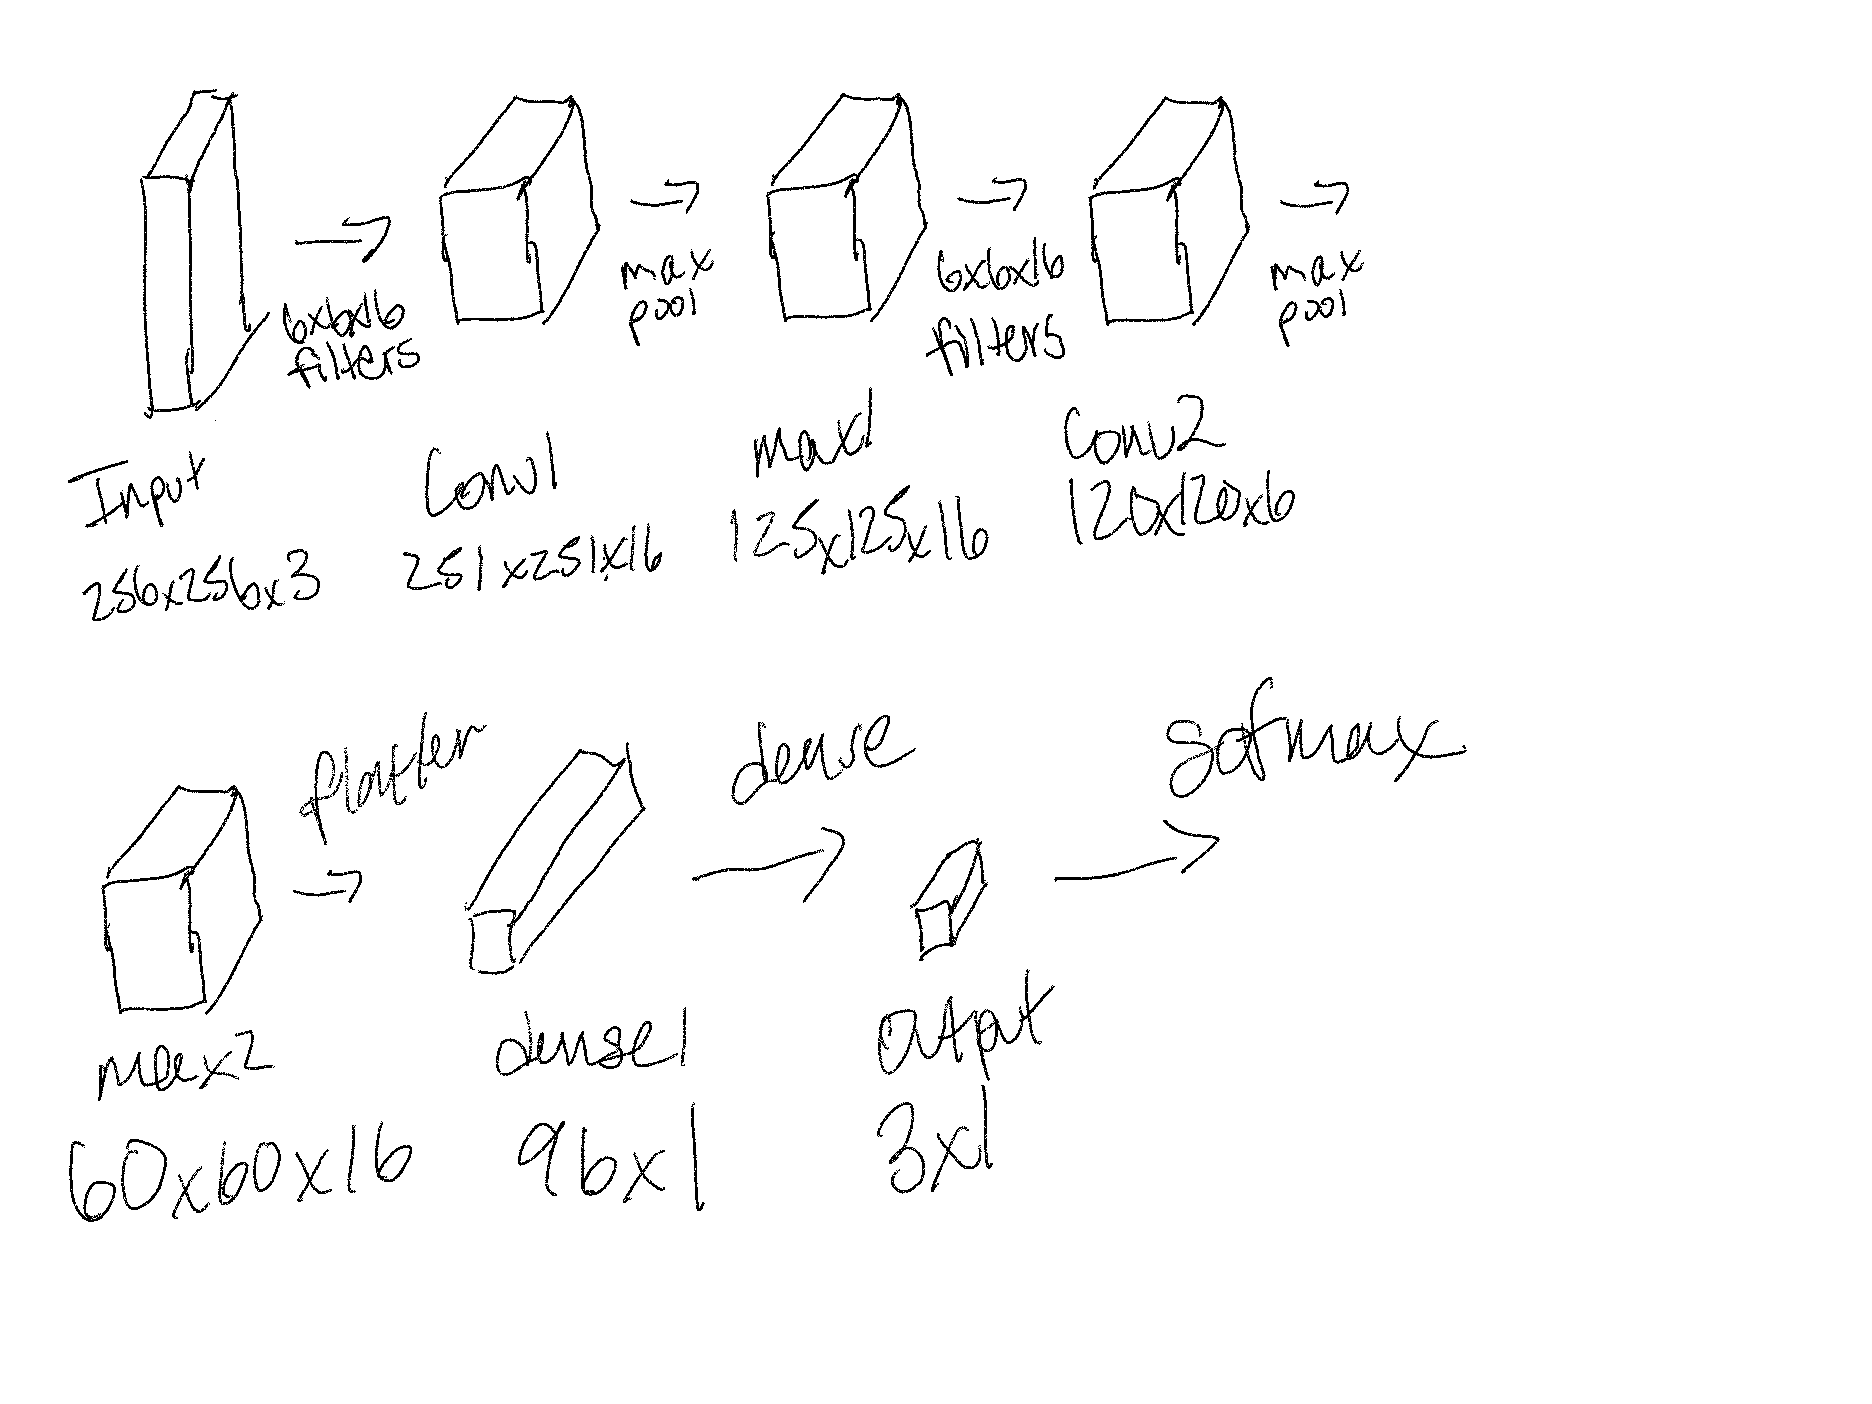
\includegraphics[width=0.8\textwidth]{assets/test2/model1.png}
              \caption{Model 1 from Question 4a}
              \label{fig:model1}
          \end{figure}

          \begin{figure}
              \centering
              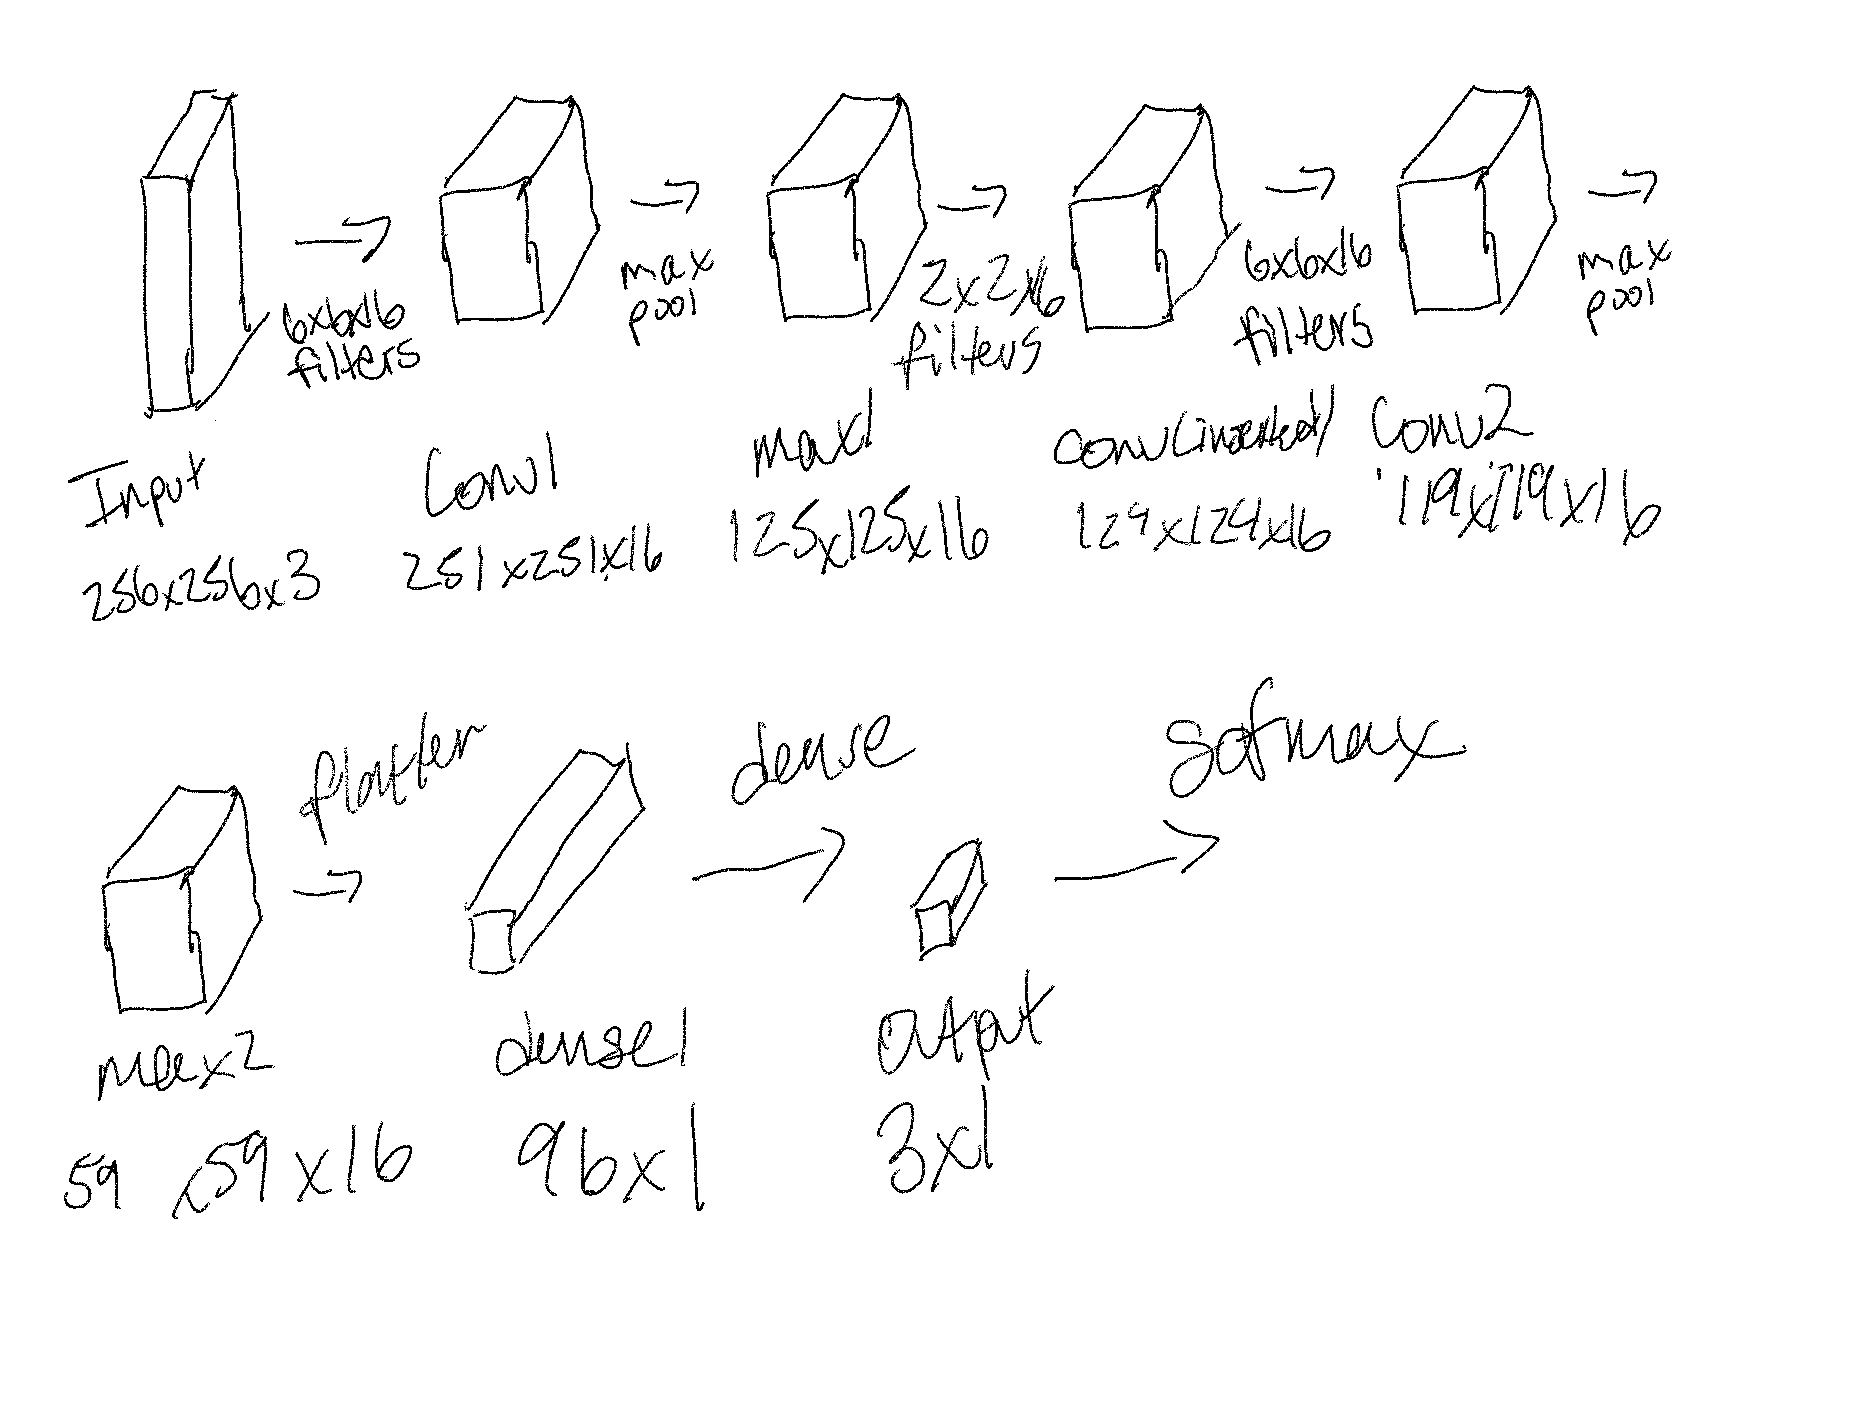
\includegraphics[width=0.8\textwidth]{assets/test2/model2.png}
              \caption{Model 2 from Question 4c}
              \label{fig:model2}
          \end{figure}
\end{enumerate}
\end{document}